The blockchain technology was first proposed in Satoshi Nakamoto’s paper, \textit{Bitcoin: A Peer-to-Peer Electronic Cash System} \cite{Nakamoto2008}, in 2008. It created a new type of digital currency, called \textit{cryptocurrency}. For example, Bitcoin \cite{bitcoin} and Ethereum \cite{ethereum} are two of the well-known cryptocurrencies. Cryptocurrencies have a significant characteristic that distinguishes them from traditional currencies: they are decentralized. This means that there is no authority in cryptocurrencies. The single authority in conventional currencies is necessary as it prevents the problem of double-spending. Therefore, the validity of transactions are important in cryptocurrencies, and it is fulfilled by consensus protocols which are based on cryptography techniques. \cite{Narayanan2016}

The major process of the blockchain systems starts with the creation of a transaction. This transaction is distributed over the blockchain network. In this state, the transaction is not-mined and therefore not persistent. Every node in the network has its own transaction pools that contain the not-mined transactions.

In a blockchain system with the proof-of-work protocol, the nodes maintain the blockchain data structure by themselves. They compete against each other in extending the blockchain by creating new blocks that persistently store transactions from the transaction pools. The addition of new blocks provides effort, since it is necessary to solve a cryptographic puzzle with the characteristic that it is hard to solve, but easy to verify given a correct solution. The solving process is called mining. A correct solution is distributed over the network and verified by the remaining network participants. In the case that the verification succeeds, the block is added to the blockchain, and the containing transactions are removed from the transaction pools.

\section{Motivation}

There are two factors that play important roles in the mining processes: the \textit{network delay} and the different \textit{mining strategies} of miners. While a transaction is published through the blockchain network, each node receives it at a different time due to characteristics of peer-to-peer networks. Therefore, each miner has different pending transactions in the transaction pool at the same time. Moreover, each miner mines a block according to the individual mining strategy simultaneously. The blocks generated by miners are different from each other, and they are also published through the unstable peer-to-peer network. Consequently, it is possible that the set of nodes partitions into different groups that work on different instances of the blockchain. These blockchains are maintained simultaneously until one blockchain becomes longer. The longest blockchain in the network is assumed to be the correct one, which is resolved by the consensus protocol.

\begin{figure}[htb]
    \centering
    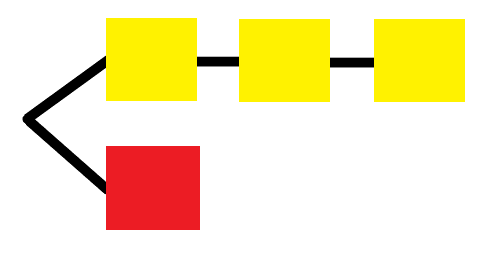
\includegraphics[width=0.7\textwidth]{intro_longest}
    \caption{Red blocks are considered to be the longest blockchain.}
    \label{fig:red blocks are considered to be the longest blockchain}
\end{figure}

For a simple example, the red blocks are the longest blockchain in Figure \ref{fig:red blocks are considered to be the longest blockchain}. There are forks on the path because of the past competitions.

In a real blockchain system, for example, there are about ten thousand of nodes in Bitcoin in April 2018 from an online statistical result \footnote{\url{https://bitnodes.earn.com/}}. For such wide and massive blockchain networks, it is hard to analyze the individual behavior of each node, e.g., the influences of the mining strategy to the mining processes under the unstable peer-to-peer network. Moreover, the mining processes of a blockchain system described earlier are dynamic and complex. Therefore, to focus on the research of the mining processes in a blockchain system, we decide to provide a visualization application to display the influences of the network delay and the mining strategy on the mining processes step by step.

\section{Methodology}

Figure \ref{fig:the method} explains the basic idea of the solution. The \textit{simulation} of the blockchain system is based on a multi-agent system, and the \textit{watchdog} monitors and records the mining activities in the blockchain system. Thus, when the transactions and the blocks are published and received by the nodes, the watchdog sends the required data to the \textit{visualizer}, which is responsible for visualizing all the mining events that happened in the blockchain system. 

\begin{figure}[htb]
    \centering
    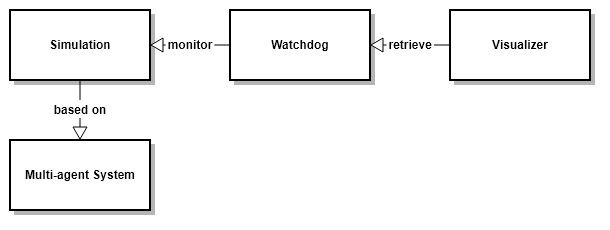
\includegraphics[width=0.8\textwidth]{intro_method}
    \caption{The method.}
    \label{fig:the method}
\end{figure}

The application is able to visualize the steps of the mining processes of each node in real-time. By setting the parameters of the network delay and the mining strategy, researchers can analyze and observe the mining processes with predefined conditions in the blockchain system. Additionally, in order to replay the same result of the blockchain processes, it is possible to provide a configuration file that defines all the properties of nodes and the parameters of the network delay and the mining strategy in the blockchain system.

\section{Contribution}

There are 8 online visualization applications, Bitbonkers, Bitnodes, BitcoinCity, Blockseer, DailyBlockchain, Elliptic, Interaqt, and Live Globe, that are summarized by Tri A. Sundara et al. \cite{Sundara2017}. Additionally, two applications, Blockchain and Etherscan, use tabular methods to represent transactions and blocks. However, these visualization applications only display the static information on Bitcoin network such as the values and the timestamps, and thus they cannot satisfy the goal which helps users to understand the dynamic mining processes. 

There are collections of previous literature that provide visualization tools to analyze the patterns of transactions on Bitcoin network. These visualization tools \cite{Kuzuno2017, Saublet2015, Fleder2015, Baumann2014} use statistical methods such as line charts, bar charts, and graph analysis to visualize the relationships and patterns of transactions and blocks. The big data visualization methods are applied \cite{McGinn2016} to find patterns of blocks. The flows of bitcoins can be tracked in the time series analysis \cite{Battista2015}. The real identification of an address can also be tracked in the analysis \cite{Kuzuno2017}. These visualization tools are implemented for analysis, though our solution focuses on visualizing the actual mining processes. 
 
Amitai Porat et al. \cite{Porat} proposed a method to analyze the potential applications of proof-of-work based blockchain networks. They considered the influences of network latency to the blockchain system. Nevertheless, our solution also considered the influences of mining strategy which are not presented in their work.

Comparing to other visualization applications and tools for blockchain systems, our solution provides the visualization of the dynamic mining processes. Furthermore, the mining processes are visualized step by step while the miners are publishing blocks through the network. Consequently, our solution is suitable for researching and understanding the complex mining processes with the factors of network delay and mining strategy.

\section{Thesis Structure}

This thesis is composed of the following chapters.

\begin{itemize}
    \item \textbf{Chapter 2} \\
        The review of the previous literature and the contribution of our approach are provided in this chapter.
    \item \textbf{Chapter 3} \\
        The assumptions and definitions of the blockchain system that the visualization is based on are given in this chapter.
    \item \textbf{Chapter 4} \\
        This chapter contains the architecture of the visualization application and the components that are implemented.
    \item \textbf{Chapter 5} \\
        In this chapter, the introduction to the usage of the visualization application is provided.
    \item \textbf{Chapter 6} \\
        Three scenarios that can be achieved by the visualization application are proposed in this chapter.
    \item \textbf{Chapter 7} \\
        At the end of this thesis, the conclusion and the future work are discussed.
\end{itemize}
